\documentclass[11pt,a4paper,oldfontcommands]{memoir}
\usepackage[utf8]{inputenc}
\usepackage[T1]{fontenc}
\usepackage{microtype}
\usepackage[dvips]{graphicx}
\usepackage{xcolor}
\usepackage{times}
\usepackage[french]{babel}




\usepackage[
breaklinks=true,
colorlinks=true,
%linkcolor=blue,urlcolor=blue,citecolor=blue,% PDF VIEW
linkcolor=black,urlcolor=black,citecolor=black,% PRINT
bookmarks=true,bookmarksopenlevel=2]{hyperref}
\usepackage[toc]{glossaries}
\makeglossaries
\usepackage{geometry}
% PDF VIEW
% \geometry{total={210mm,297mm},
% left=25mm,right=25mm,%
% bindingoffset=0mm, top=25mm,bottom=25mm}
% PRINT
\geometry{total={210mm,297mm},
left=20mm,right=20mm,
bindingoffset=0mm, 
top=25mm,bottom=25mm}

\OnehalfSpacing
%\linespread{1.3}

%%% CHAPTER'S STYLE
%\chapterstyle{bianchi}
%\chapterstyle{ger}
\chapterstyle{madsen}
%\chapterstyle{ell}
%%% STYLE OF SECTIONS, SUBSECTIONS, AND SUBSUBSECTIONS
\setsecheadstyle{\Large\bfseries\sffamily\raggedright}
\setsubsecheadstyle{\large\bfseries\sffamily\raggedright}
\setsubsubsecheadstyle{\bfseries\sffamily\raggedright}


%%% STYLE OF PAGES NUMBERING
%\pagestyle{companion}\nouppercaseheads 
%\pagestyle{headings}
%\pagestyle{Ruled}
\pagestyle{plain}
\makepagestyle{plain}
%\makeevenfoot{plain}{\thepage}{}{}
\makeevenfoot{plain}{}{}{\thepage}
\makeoddfoot{plain}{}{}{\thepage}
\makeevenhead{plain}{}{}{}
\makeoddhead{plain}{}{}{}


\maxsecnumdepth{subsection} % chapters, sections, and subsections are numbered
\maxtocdepth{section} % chapters, sections, and subsections are in the Table of Contents


%%%---%%%---%%%---%%%---%%%---%%%---%%%---%%%---%%%---%%%---%%%---%%%---%%%


\begin{document}

%%%---%%%---%%%---%%%---%%%---%%%---%%%---%%%---%%%---%%%---%%%---%%%---%%%
%   TITLEPAGE
%
%   due to variety of titlepage schemes it is probably better to make titlepage manually
%
%%%---%%%---%%%---%%%---%%%---%%%---%%%---%%%---%%%---%%%---%%%---%%%---%%%
\thispagestyle{empty}

{%%%
\sffamily
\centering
\Large
Université de Nantes\\
Faculté des sciences et Techniques\\
M1 ALMA - Architecture Logicielle\\



~\vspace{\fill}

{\huge 
\textbf{Mini editeur de texte en Scala}
}

\vspace{4cm}

{\LARGE
Alexis Ruchaud\\
Muriel Cadiot
}\\


\vspace{3.5cm}

Dossier de conception\\[1em]
%[0.5em]


\vspace{3.5cm}



\vspace{\fill}

Decembre 2014

%%%
}%%%

%\cleardoublepage
%%%---%%%---%%%---%%%---%%%---%%%---%%%---%%%---%%%---%%%---%%%---%%%---%%%
%%%---%%%---%%%---%%%---%%%---%%%---%%%---%%%---%%%---%%%---%%%---%%%---%%%
\clearpage
\tableofcontents*


\clearpage
\chapter{Introduction}
\section{Presentation du projet}

Ce projet consiste en la création d'un editeur de texte proposant à l'utilisateur différentes fonctionnalités. L'application a été réalisée en Scala à l'aide de l'IDE Eclipse tandis que les diagrammes de conception ont été créés à l'aide du plugin Eclipse Papyrus.\\
Le mini éditeur de texte permet à l'utilisateur d'entrer du texte dans une zone de travail (Buffer) et de réaliser différentes actions sur ce dernier. Ces actions sont celles que l'on peut retrouver dans la plupart des editeurs de texte : la possibilité de sélectionner du texte, de le copier/couper, de le coller et des fonctions pour annuler un changement ou d'en rétablir un précedemment annulé. Ces commandes pourront être groupées sous forme de macro afin de permettre à l'utilisateur de créer lui même des commandes personnalisées afin de faciliter son travail.

\section{Organisation du document}
Pour présenter ce projet nous étudierons tout d'abord la partie analyse et conception de l'application en commençant par la problématique du projet en présentant un cas d'utilisation expliquant les possibilités de l'utilisateur. Nous verrons ensuite différents diagrammes de classe représentant le projet. Enfin nous observerons avec un diagramme de séquence l'exécution d'une commande du mini editeur.\\
Dans une deuxième partie nous présenterons la partie développement de l'application en présentant les classes du projet ainsi que leur rôle.\\
Enfin nous concluerons sur les perspectives du projet en présentant les différentes améliorations possibles du mini editeur.

\chapter{Analyse et conception}
\section{Cas d'utilisation}
Le cas d'utilisation suivant illustre l'utilisation d'une commande. Lorsque l'utilisateur exécute une commande il appelle la classe mère "Command" qui selon l'objet utilisé appel la commande correspondante. De plus le lien "include" reliant la commande à "Save" indique qu'une sauvegarde du Buffer sera réalisée à chaque exécution d'une commande. Cette sauvegarde ce fait à l'aide du patron de conception Memento. \\
\begin{figure}[!ht]
\centering 
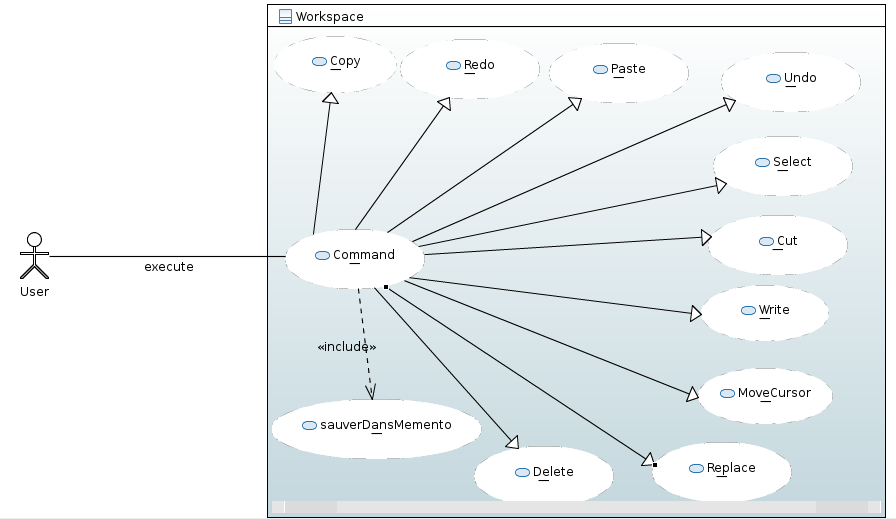
\includegraphics[width=13cm]{useCaseCommand.png}
\caption{UseCase : Command}
\label{figure1}
\end{figure}
\section{Diagrammes de classe}
Dans cette section, nous mettrons en avant les diagrammes de classes des différents patrons de conception qui sont contenus dans le mini éditeur de texte.
Nous avons choisi de montrer en priorité ces diagrammes car ils sont l'angle le plus intéressant par lequel observer le programme. Vous trouverez en annexe le diagramme de classe complet de l'application.
\subsection{Command pattern}
Le pattern command est un patron de conception permettant de séparer le code appellant une action de l'action elle même. Il permet entre autres la création d'interface réalisant des commandes de tel façon que l'interface ne connaisse pas l'action réalisée par la commande. \\
Un éditeur de texte possèdant de nombreuses commandes (Copy , Cut , Undo etc..) il nous a semblé naturel de choisir ce pattern dans la création de l'application. En plus de l'encapsulation fournie par ce pattern, son utilisation nous permettra au besoin de créer de nouvelles commandes très facilement sans avoir a modifier/ajouter beaucoup de code.
\begin{figure}[!ht]
\centering 
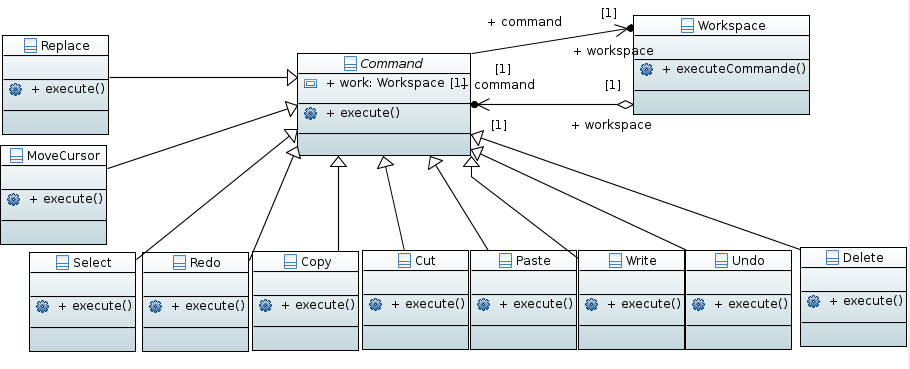
\includegraphics[width=13cm]{CommandPattern.png}
\caption{Command pattern}
\label{figure2}
\end{figure}
\subsection{Memento Pattern}
Le patron de conception Memento permet de créer des objets permettant de sauvegarder et de restaurer l'état interne d'un programme à un moment donné.
Notre éditeur de texte comportant des commandes \emph{Undo} et \emph{Redo} l'utilisation de ce pattern nous a grandement facilité la tâche pour la réalisation de ces fonctions. Voici le diagramme de ce patron de conception.\footnote{Le type de Gardien.listMemento est une liste de memento, nous avons laissé le champ indéfini car nous n'avons pas trouvé comment faire un type ListBuffer dans Papyrus}
\begin{figure}[!ht]
\centering 
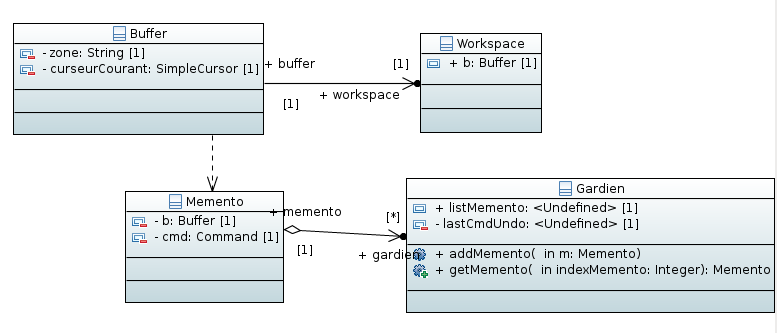
\includegraphics[width=13cm]{MementoPattern.png}
\caption{Memento Pattern}
\label{figure3}
\end{figure}
\subsection{Composite Pattern}
Le pattern composite permet la création de structure contenant des objets avec des comportements communs. Dans notre cas, nous avons utilisé le pattern composite pour permettre a l'utilisateur de créer des macros. Grâce au composite, l'utilisateur pourra manipuler une liste de commande de la même façon qu'une commande. La seule différence sera que toute les commandes de la liste seront exécutées lors de l'appel de la macro.\footnote{Ici listCommand est du type ListBuffer<Command>}
\begin{figure}[!ht]
\centering 
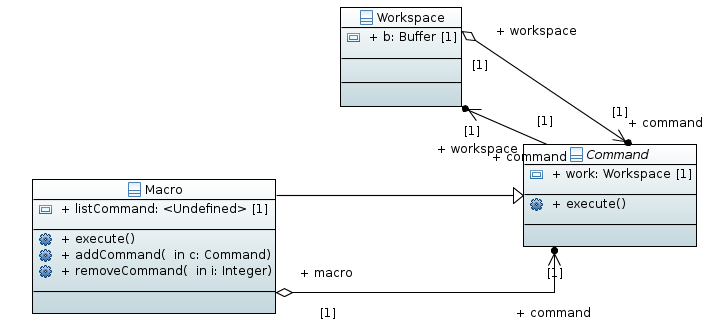
\includegraphics[width=13cm]{CompositePattern.png}
\caption{Composite Pattern }
\label{figure4}
\end{figure}
\subsection{Observer Pattern}
Le pattern observer permet de créer un objet qui en observera un autre et effectuera une opération lors du changement de celui-çi. Lorsque l'objet observé est modifié, les observateurs recoivent une notification et effectuent une action. Dans notre cas le pattern Observer s'applique sur le Workspace, quand ce dernier est modifié par une commande, l'observateur est notifié et appel un affichage du buffer\footnote{Ici observers est du type ListBuffer<Observer>}. \\
\begin{figure}[!ht]
\centering 
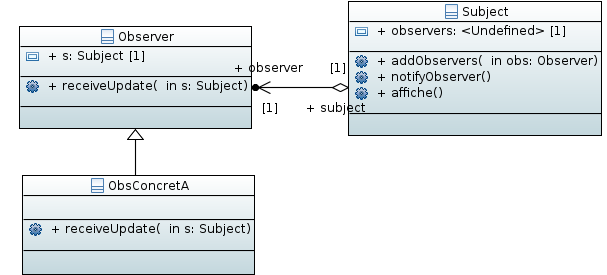
\includegraphics[width=13cm]{ObserverPattern.png}
\caption{Observer Pattern }
\label{figure5}
\end{figure}
\section{Diagramme de séquence}
Nous allons présenter ici un diagramme de séquence représentant l'action utilisateur \emph{Write}.\\
Pour appeler la commande Write, il faut tout d'abord créer un objet Command de type Write que l'on transmet au Workspace. Celui-çi ce charge de lancer l'exécution de la commande en l'envoyant à la classe Write. Une fois le message de retour arrivé, le Workspace notifie les utilisateurs du changement qui a eu lieu. Le buffer récupère la notification avec sa méthode \emph{receiveUpdate()} ce qui déclanche l'affichage. \\
L'exécution des autres commandes fonctionnant de la même manière que la commande \emph{Write}, nous ne présenterons sous forme de diagramme de séquence que ce cas la. \\
\begin{figure}[!ht]
\centering 
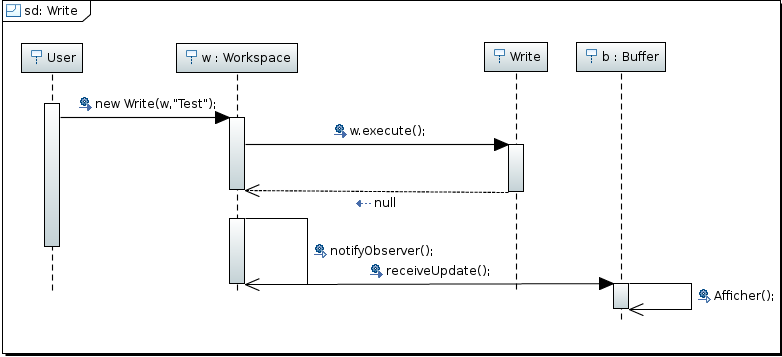
\includegraphics[width=13cm]{diagSeq.png}
\caption{Diagramme de sequence : Write}
\label{figure6}
\end{figure}
\\

\chapter{Developpement}
Dans cette section nous présenterons les classes contenant l'application en expliquant rapidement leur fonction.\\
\begin{description}
  \item[Buffer] La classe Buffer représente la zone de texte sur laquelle travaille l'utilisateur.
  \item[ClipBoard] Le ClipBoard est la classe où l'on stocke la sélection après avoir copié ou coupé.
  \item[Command] La classe abstraite Command est la classe mère des commandes concrètes.
  \item[Copy] Copy hérite de Command et permet de copier une sélection dans le ClipBoard.
  \item[Cursor] Cursor est la classe mère de SimpleCursor et DoubleCursor.
  \item[Cut] Cut hérite de Command et permet de couper une string sélectionnée et de la mettre dans le ClipBoard.
  \item[Delete] Delete hérite de Command et permet de supprimer une string sélectionnée du Buffer.
  \item[DoubleCursor] DoubleCursor hérite de Cursor et permet de délimiter à l'aide de deux entiers une châine de caractère à l'interieur du buffer.
  \item[Gardien] Le Gardien est la classe chargée de garder en mémoire l'historique du Buffer ainsi que de renvoyer une version plus ancienne de ce dernier.
  \item[Macro] La classe Macro hérite de Command. Elle fonctionne de la même manière que les autres commandes à la différence près qu'elle exécute une liste de commande.
  \item[Memento] La classe Memento permet de créer des historiques du Buffer qui seront stockés dans le Gardien.
  \item[MoveCursor] MoveCursor hérite de Command et permet de déplacer le curseur courant afin d'insérer du texte ailleurs qu'à la fin du buffer.
  \item[ObsConcretA] ObsConcretA hérite de Observer et permet d'afficher le buffer lors de la notification de modification de ce dernier.
  \item[Observer] Classe mère de ObsAffiche.
  \item[Paste] Paste hérite de Command et permet de coller le contenu du ClipBoard à la position du curseur courant dans le buffer.
  \item[Redo] Redo hérite de Command et permet de remettre en place la dernière action annulée avec Undo.
  \item[Replace] Replace hérite de Command et permet de remplacer la sélection par le contenu du ClipBoard.
  \item[Selection] La classe Sélection contient la chaîne de caractère située entre les curseurs de DoubleCursor.
  \item[Selectionner] Hérite de Command et permet de sélectionner une partie du buffer.
  \item[SimpleCursor] Hérite de Cursor et représente le curseur courant du buffer.
  \item[Subject] Contient la liste des observeurs et permet de les notifier lors d'un changement du buffer.
  \item[Undo] Undo hérite de Command et permet d'annuler la dernière action réalisée.
  \item[Workspace] Workspace contient le buffer, le ClipBoard et est la classe ou sont appelées les commandes.
  \item[Write] Write hérite de Command et permet de demander à l'utilisateur d'entrer une chaîne de caractère pour l'ajouter dans le buffer.
\end{description}
\chapter{Bilan}
\section{Conclusion}
Le langage de programmation Scala étant totalement nouveau pour nous, l'implémentation de l'application a pris plus de temps qu'il nous en aurait fallu avec un langage que nous connaissions. Il reste néanmoins avantageux d'avoir pu travailler sur un langage inconnu ne serait ce que pour la connaissance personnelle. En effet il est toujours intéressant d'avoir des bases dans de nombreux domaines afin de ne pas se retrouver désamparer lors d'un travail sur un de ces domaines. \\
De même l'utilisation de Papyrus était totalement nouvelle, nous avions jusque la toujours utilisé des logiciels exterieurs à Eclipse qui n'était pas toujours conforme à la norme UML. Le fait que Papyrus soit directement lié à l'IDE permet de mieux lier la conception du projet avec son implementation.\\
Enfin l'utilisation de patron de conception pour la réalisation de certaines fonctionnalités nous ont grandement facilité la tâche. En plus de cela, la présence de patron de conception dans le code donne une capacité d'extensibilité à l'application.
\section{Perspectives}
Bien que respectant les consignes données en début de projet, de nombreuses améliorations de l'application reste possible.\\
Tout d'abord, avec une connaissance plus approfondie du langage Scala nous pourrions réecrire une grande partie du code dans un but d'optimisation et d'un meilleur respect de l'aspect Génie Logiciel de l'implémentation.\\
Un ajout d'une interface graphique au projet serait aussi une amélioration importante possible afin de rendre l'utilisation du mini éditeur de texte plus simple.\\
Enfin il reste de nombreuses améliorations que l'on peut retrouver dans les éditeurs de texte dit standarts qui pourraient être implémentés dans ce projet.\\
En conclusion, il reste de nombreuses pistes d'améliorations qui pourraient être suivies : au niveau des fonctionnalités, de l'implémentation ou de la conception
\appendix
\chapter{Annexe}
\begin{figure}[!ht]
\centering 
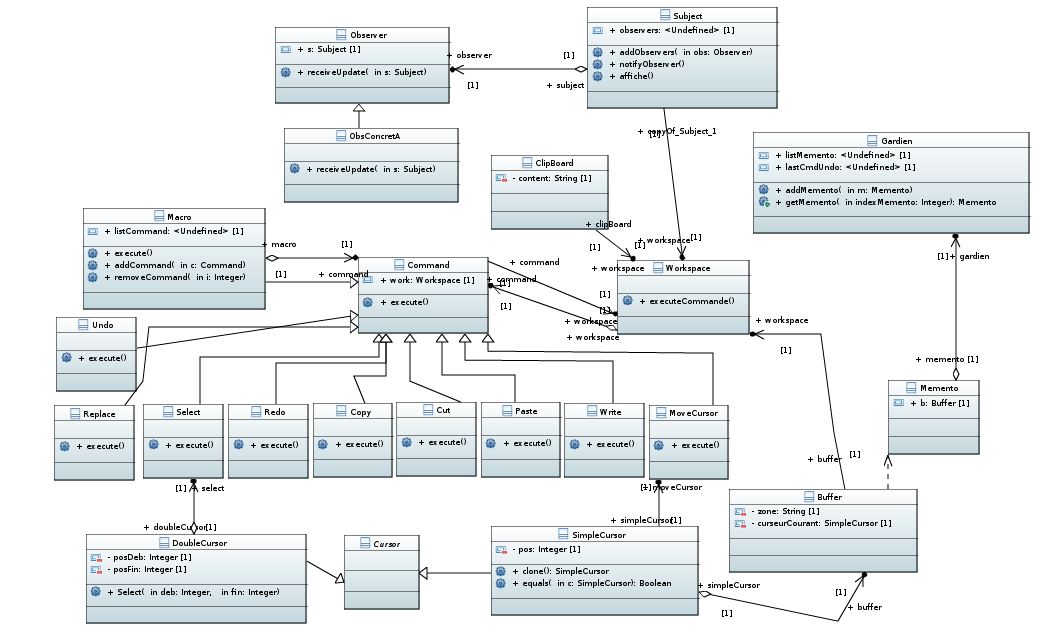
\includegraphics[angle=90,width=10cm]{CompletDiagram.png}
\caption{Diagramme UML de l'application}
\label{figure7}
\end{figure}
\end{document}
